\documentclass{erauthesis}
\department{Mechanical Engineering}
\chair{Eric Coyle, Ph.D}
\dean{James Gregory, Ph.D.}
\dgc{Lon Moeller, J.D.}
\depchair{Patrick Currier, Ph.D.}
\advisortitle{Committee chair}
\usepackage{graphicx}
\usepackage{amsmath}
\usepackage{amssymb}
\usepackage{textcomp, gensymb}
\usepackage{array}
\usepackage{enumitem}
\usepackage{xcolor}
\usepackage{algorithm}
\usepackage{algpseudocode}

\usepackage{subcaption} % for multiple image figures
% \usepackage[style=authoryear]{biblatex} % or numeric, apa, etc.
% \addbibresource{Dissertation.bib}         % your Zotero export

% pkgs for .mermaid chart
\usepackage{tikz}
\usetikzlibrary{shapes.geometric, arrows}

% acronyms
\usepackage[nolist]{acronym} 

% preamble for Lit-review tables:
\usepackage{tabularx,ragged2e,makecell}
\renewcommand\theadfont{\bfseries}
\renewcommand\cellalign{tl} % top-left for makecell
\newcolumntype{L}[1]{>{\RaggedRight\arraybackslash}p{#1}}
\newcolumntype{Y}{>{\RaggedRight\arraybackslash}X}

\title{A STUDY IN OBJECT DETECTION AND CLASSIFICATION
PERFORMANCE BY SENSING MODALITY FOR AUTONOMOUS
SURFACE VESSELS} % the title should be included here
\author{Daniel P. Lane} 
\graduation{December}{2025}
\advisor {Eric Coyle} %Committe chair


\coadvisor{Subhradeep Roy} % If you do not have a co-advisor, delete this whole command

\committememzero{Xxxx X. Xxxxxxxxx, Ph.D.} % If you have a co-advisor, do not edit this member name
%% Enter the name of the committee members
\committememone{Patrick Currier}
\committememtwo{Monica Garcia}
\committememthree{Jianhua Liu}
\committememfour{TBD}



%\signaturepush{-2.0}									

\usepackage{subfiles} % Best loaded last in the preamble

\begin{document}


\frontmatter

\maketitle

% \makesignature
\makeatletter 
\advance\fau@frontstage by 1  % Skip signature page but maintain counter
% \makeanother
\begin{acronym}[GB-CACHE] % Give the longest label here so that the list is nicely aligned
\acro{AGS}{autonomous ground system}
\acro{ASV}{autonomous surface vessel}
\acro{USV}{unmanned surface vessel}
\acro{ERAU}{Embry-Riddle Aeronautical University}
\acro{GB-CACHE}{grid-based clustering and concave hull extraction}
\acro{GPS}{Global Positioning System}
\acro{WAM-V}{wave-adaptive modular vessel}
\acro{SDR}{standard dynamic range}
\acro{HDR}{high dynamic range}
\acro{DOL-HDR}{digital-overlap HDR}
\acro{IMU}{inertial measurement unit}
\acro{INS}{inertial navigation system}
\acro{IoU}{intersection over union}
\acro{LiDAR}{light detection and ranging}
\acro{pps}{points per second}
\acro{mAP}{mean average precision}
\acro{MPC}{model predictive control}
\acro{RGB}{red, green, blue}
\acro{ROI}{region of interest}
\acro{ROS}{Robot Operating System}
\acro{YOLO}{You Only Look Once}
\acro{YOLOv8}{You Only Look Once ver. 8.0}
\acro{LWIR}{long-wave infrared}
\acro{FPS}{frames per second}
\acro{EFL}{effective focal length}
\acro{FOV}{field of view}
\acro{LAN}{local area network}
\acro{SEI}{supplemental enhancement information}
\acro{NAL}{network abstraction layer}
\acro{NTP}{Network Time Protocol}
\acro{PTP}{Precision Time Protocol}
\acro{RTP}{Real-time Transport Protocol}
\acro{RTSP}{Real-time Streaming Protocol}
\acro{UDP}{User Datagram Protocol}

\end{acronym}

\begin{acknowledgements}
% \raggedright
I would like to express my deepest gratitude to my friends, family, and especially my parents, whose unwavering love, encouragement, and support have sustained me throughout my academic journey. Their belief in me has been a constant source of strength and motivation.

I am sincerely thankful to my advisor, Dr. Coyle, for his mentorship and steady guidance throughout this research. He has taught me lessons both in and beyond the classroom that will stay with me for a lifetime, and for that, I will be forever grateful.

I would also like to extend a special thanks to my co-advisor, Dr. Roy, who first introduced me to the world of academic research rigor. His guidance shaped the foundation of my development as a researcher and helped me grow into the kind of professional and scholar I aspired to become.

Finally, I wish to acknowledge the faculty and staff of the Department of Mechanical Engineering for their continued support of my academic and professional growth. 
Their commitment to excellence in teaching and research has profoundly influenced my development as both a student and an educator.

\vspace{3mm}

This work was supported in part by NEEC grant N00174-22-1-0012 through NUWC Keyport.
Any opinions, findings, conclusions, or recommendations expressed in this material are those of the authors and do not necessarily reflect the views NUWC Keyport or
the Department of the Navy.
\end{acknowledgements}

\begin{abstract}
	% \raggedright Researcher: Daniel P. Lane
 % \\Title: A study in object detection and classification performance by sensing modality for autonomous surface vessels \\Institution:	Embry-Riddle Aeronautical University\\Degree:	Doctor of Philosophy in Mechanical Engineering\\Year:	2025 \\
 This research addresses the critical gap in quantitative performance comparison between \ac{LiDAR} and vision-based sensing for real-time maritime object detection on autonomous surface vessels.
 Using \ac{ERAU}'s Minion platform and 2024 Maritime RobotX Challenge data, this study evaluates \ac{GB-CACHE} \ac{LiDAR} processing against \ac{YOLO} vision detection across six maritime object categories. The methodology encompasses real-time performance analysis, multi-sensor calibration, and sensor fusion for bounding box confidence integration.
 Performance metrics include precision, recall, \ac{mAP}, training requirements, and computational efficiency. 
 % Results demonstrate [key performance finding] and establish [fusion outcome]. 
 The research provides quantitative baselines for maritime sensing modality selection and validated calibration procedures enabling improved autonomous navigation in complex maritime environments.

%%%% Coyle Note: %%%%
% this study evaluates LiDAR and vision-based detection and classification acrsoss six maritime object categories, using GB-CACHE and Yolov8 as representative processing techniques for each modality.

\end{abstract}
\pagetableofcontents
\clearpage
\listoftables					% Or \nolistoftables if there are no 
\clearpage
\listoffigures					% Or \nolistoffigures if there are no 




\mainmatter
\newpage
\chapter{Introduction} \label{introduction}
\subfile{sections/introduction_02}
% \section{Significance of Study} \label{significance_of_study}
% \subfile{sections/significance_of_study}
% \section{Problem Statement: Performance Comparison Gap} \label{problem_statement1}
% \subfile{sections/problem_statement1}

% \chapter{Introduction} \label{ch:introduction}

% % \section{Background and Motivation}
% The rise of autonomous systems is transforming numerous industries, and the maritime sector is no exception. 
% Autonomous surface vessels (ASVs) have the potential to enhance operational safety by performing dull, dirty, and dangerous tasks traditionally handled by humans. 
% A critical enabler of these capabilities is reliable environmental perception. Real-time object detection and classification underpin autonomous navigation and situational awareness, ensuring that vessels can respond safely to dynamic maritime conditions.

% While the automotive industry has achieved substantial progress in perception and control for autonomous vehicles, comparable developments in maritime autonomy remain limited. 
% This disparity is reflected in the relative volume of published research: automotive detection strategies are extensively studied, whereas maritime detection and classification methods are less mature. 
% Although detection algorithms from the automotive domain can be adapted for ASVs, direct translation is nontrivial. 
% The maritime domain is inherently less structured, with dynamic, unbounded scenes and significant environmental variability, especially in littoral regions.

% % \section{Challenges in Maritime Perception}
% Maritime object detection presents distinct challenges absent from land-based environments. 
% Turbulent wave motion, specular reflections, atmospheric haze, and fluctuating illumination conditions degrade visual and ranging sensor performance. 
% Conventional marine radar provides extended range but insufficient spatial resolution for close- and mid-range perception. 
% Cameras and LiDAR sensors offer denser data but remain sensitive to lighting and weather conditions. 
% These factors necessitate sensor fusion approaches capable of combining complementary information from multiple sensing modalities to enhance robustness and reliability. 
% However, optimal real-time fusion strategies for maritime applications remain an open research problem.

% % \section{Problem Statement}
% Despite recent advances in both LiDAR- and camera-based perception, autonomous surface vessels continue to face significant limitations in real-time object detection and classification. 
% Existing solutions often rely on single-modality sensing or are adapted from automotive systems without full consideration of maritime dynamics, environmental conditions, or computational constraints. 
% There is a need for validated fusion frameworks that integrate spatial and temporal calibration with efficient detection pipelines to enable reliable perception on embedded maritime platforms.

% % \section{Knowledge Gap}
% Prior research demonstrates the potential of multimodal fusion in terrestrial and aerial robotics, but only limited experimental work has been conducted using real-world maritime datasets. 
% Many studies focus on simulated or controlled environments, and few address real-time performance constraints or synchronization between sensors. 
% Consequently, there is insufficient understanding of how LiDAR and camera modalities complement one another under operational maritime conditions, and how their integration affects detection accuracy, computational load, and latency.

% % \section{Research Objectives}
% Within the domain of surface-level maritime perception under daylight and near-optimal conditions, this research aims to:
% \begin{enumerate}
%     \item Develop and validate spatial and temporal calibration frameworks for LiDAR–camera fusion that achieve sub-pixel projection accuracy and maintain synchronization latency below 150~ms.
%     \item Quantitatively compare the independent performance of visual and LiDAR-based detection networks by:
%     \begin{itemize}
%         \item Assessing the training data requirements for accurate classification across modalities,
%         \item Evaluating detection and classification performance across maritime object classes that exhibit geometric and visual variability, and
%         \item Identifying the complementary strengths of each sensing modality for integration in fusion architectures.
%     \end{itemize}
%     \item Design, implement, and benchmark early, mid, and late fusion frameworks to evaluate:
%     \begin{itemize}
%         \item Computational efficiency and end-to-end detection latency,
%         \item Classification accuracy of fused modalities, and
%         \item Performance tradeoffs relevant to embedded maritime ASV platforms.
%     \end{itemize}
% \end{enumerate}

% % \section{Scope of the Research}
% This study focuses on detecting and classifying maritime objects such as buoys, navigational markers, and small to medium-sized watercraft using LiDAR and HDR camera sensors integrated on Embry-Riddle Aeronautical University’s \textit{Minion} ASV platform. 
% Data are collected under controlled and open-water conditions, limited to daylight hours and clear weather to isolate the effects of sensor modality rather than environmental degradation. Evaluation emphasizes real-time performance and comparative accuracy rather than extreme-weather resilience or multi-vessel coordination.

% % \section{Methodological Overview}
% The research employs a comparative framework that evaluates each sensing modality independently and within fused configurations. The visual detection pipeline utilizes a fine-tuned YOLO network, while LiDAR-based detection applies the GB-CACHE clustering and classification algorithm. 
% Fusion strategies are implemented within the Robot Operating System (ROS) to ensure reproducible timing and message synchronization through recorded bag files. 
% Detection performance is quantified using precision, recall, and intersection-over-union (IoU) metrics, while computational load and latency are measured through CPU, GPU, and memory utilization during real-time inference.

% % \section{Expected Contributions}
% This dissertation contributes to the field of maritime perception through:
% \begin{enumerate}
%     \item A validated calibration and synchronization framework for LiDAR–camera fusion on embedded ASV systems.
%     \item A quantitative evaluation of modality-specific and fused detection networks using real-world maritime data.
%     \item A performance benchmarking methodology that integrates accuracy, latency, and computational efficiency metrics for real-time ASV perception.
%     \item Recommendations for selecting and deploying fusion strategies optimized for resource-constrained maritime platforms.
% \end{enumerate}

% % \section{Dissertation Structure}
% The remainder of this dissertation is organized as follows.  
% Chapter~\ref{litReview} reviews related work on maritime sensing, multimodal fusion, and real-time object detection frameworks.  
% Chapter~\ref{sensing_platform} details the sensing hardware and system architecture of the Minion ASV platform.  
% Section~\ref{sec:calibration} presents spatial and temporal calibration methodologies.  
% Chapter~\ref{realtime_object_detection} discusses the visual and LiDAR detection algorithms and their fusion strategies.  
% Section~\ref{detect_results} reports performance results and analyzes comparative findings.  
% Finally, Chapter~\ref{chap:recommendations} summarizes contributions and outlines future research directions.

%%%%%%%%%%%%%%%%%%%%%%%%%%%%%%%%%%%%%%%%%%%%%%%%%%%
%%%%%%%%%%%%%%%%%%%%%%%%%%%%%%%%%%%%%%%%%%%%%%%%%%%
%%%%%%%%%%%%%%%%%%%%%%%%%%%%%%%%%%%%%%%%%%%%%%%%%%%
\chapter{Literature Review} \label{litReview}
% \subfile{sections/literatureReview_new}
\subfile{sections/literatureReview_v07_md}

%%%%%%%%%%%%%%%%%%%%%%%%%%%%%%%%%%%%%%%%%%%%%%%%%%%
%%%%%%%%%%%%%%%%%%%%%%%%%%%%%%%%%%%%%%%%%%%%%%%%%%%
%%%%%%%%%%%%%%%%%%%%%%%%%%%%%%%%%%%%%%%%%%%%%%%%%%%
\chapter{Sensing Platform} \label{sensing_platform}
\subfile{sections/sensing_platform_intro}

\section{Perception Geometry} \label{perception_geometry}
\subfile{sections/perception_geometry}

\section{Sensors} \label{sensors}
% \subfile{sections/sensors}

\subsection{LiDAR} \label{sensors_LiDAR}
\subfile{sections/LiDAR}

\subsection{Visible Spectrum Cameras} \label{visual_cameras}
\subfile{sections/cameras}

\subsection{PinPoint GPS/INS} \label{sensors_GPS}
\subfile{sections/pinpoint}

\section{Networking and Computing Hardware} \label{sec:Atlas_LAN}
\subfile{sections/hardware}

\section{Sensor Calibration} \label{sec:calibration}
\subfile{sections/calibration}

\begin{figure}[htbp]
    \centering
    \includegraphics[width=0.7\linewidth]{Images/tf_tree_1.png}
    \caption{Transform hierarchy for Minion: the GPS-defined \texttt{map} frame anchors the ROS TF tree used for LiDAR–camera projection and sensor fusion.}
    \label{fig:tf_tree}
\end{figure}

%%%%%%%%%%%%%%%%%%%%%%%%%%%%%%%%%%%%%%%%%%%%%%%%%%%%%%%%%%%%%%%%%%%%
\subsection{Spatial Calibration} \label{spatial_calibration}

Before data from the camera and \ac{LiDAR} sensors can be combined, each device must be spatially calibrated through intrinsic and extrinsic transformations.  
This process establishes the geometric relationships required to express all sensor measurements in a unified coordinate frame, enabling accurate projection of \ac{LiDAR} points onto the camera image plane.

Calibration begins with determining the camera’s intrinsic parameters, followed by estimation of the extrinsic transformation that defines the rigid-body relationship between the camera and each \ac{LiDAR} sensor.  
The following sections describe the methods and results of this calibration process.

%%%%%%%%%%%%%%%%%%%%%%%%%%%%
\subsubsection{LiDAR Extrinsic Calibration} \label{extrinsic_tform}
\subfile{sections/extrinsic_tform}

\begin{figure}[htbp]
    \centering
    \includegraphics[width=0.9\linewidth]{Images/Lidar2Lidar.png}
    \caption{Example of LiDAR–LiDAR alignment.}
    \label{fig:Lidar2Lidar}
\end{figure}

\subsubsection{LiDAR Calibration Results} \label{results_lidarLidar_calib}
\subfile{sections/results_lidarlidar}

\begin{figure}[ht]
\centering
        \includegraphics[width=0.95\textwidth]{Images/livox_viewer.png} 
\caption{Data from port (red), center (green), and starboard (yellow) Livox Units as viewed within the Livox Viewer software (left), and the integrated calibration tool with estimated extrinsic parameters shown (right). }
\label{fig:LidarLidar_calib}
\end{figure}


%%%%%%%%%%%%%%%%%%%%%%%%%%%%
\subsubsection{Camera Intrinsics} \label{camera_intrinsics}
\subfile{sections/cam_intrinsics}

\begin{figure}[htbp]
\centering
\makebox[\textwidth][c]{%
    \begin{subfigure}[t]{0.3\textwidth}
        \centering
        \includegraphics[width=\textwidth]{Images/cam_calib_1.png}
        \caption{A single example of detected and reprojected checkerboard corners.}
        \label{fig:cam_calib_1}
    \end{subfigure}
    \hspace{2em}
    \begin{subfigure}[t]{0.625\textwidth}
        \centering
        \includegraphics[width=\textwidth]{Images/cam_calib_2.png}
        \caption{Reprojection of sample target poses into the 3D world frame after calibration.}
        \label{fig:cam_calib_2}
    \end{subfigure}%
}
\caption{Checkerboard images are processed to detect corners. Agreement between detected (green circles) and reprojected (red crosses) points demonstrates corner localization and mapping of the image coordinate system.(left), which enable intrinsic parameters to be estimated and validated by reprojecting known targets into three-dimension space (right).}
\label{fig:cam_calib}
\end{figure}

\subsubsection{Camera Calibration Results} \label{sec:camera_intriniscs_results}
\subfile{sections/cam_intrinsics}

\begin{figure}[htbp]
    \centering
    \includegraphics[width=0.9\linewidth]{Images/checkerboard_old.jpg}
    \caption{Older paper-based checkerboards maintained dimensional accuracy but degraded over time.}
    \label{fig:checkerboard_old}
\end{figure}

\begin{figure}[htbp]
    \centering
    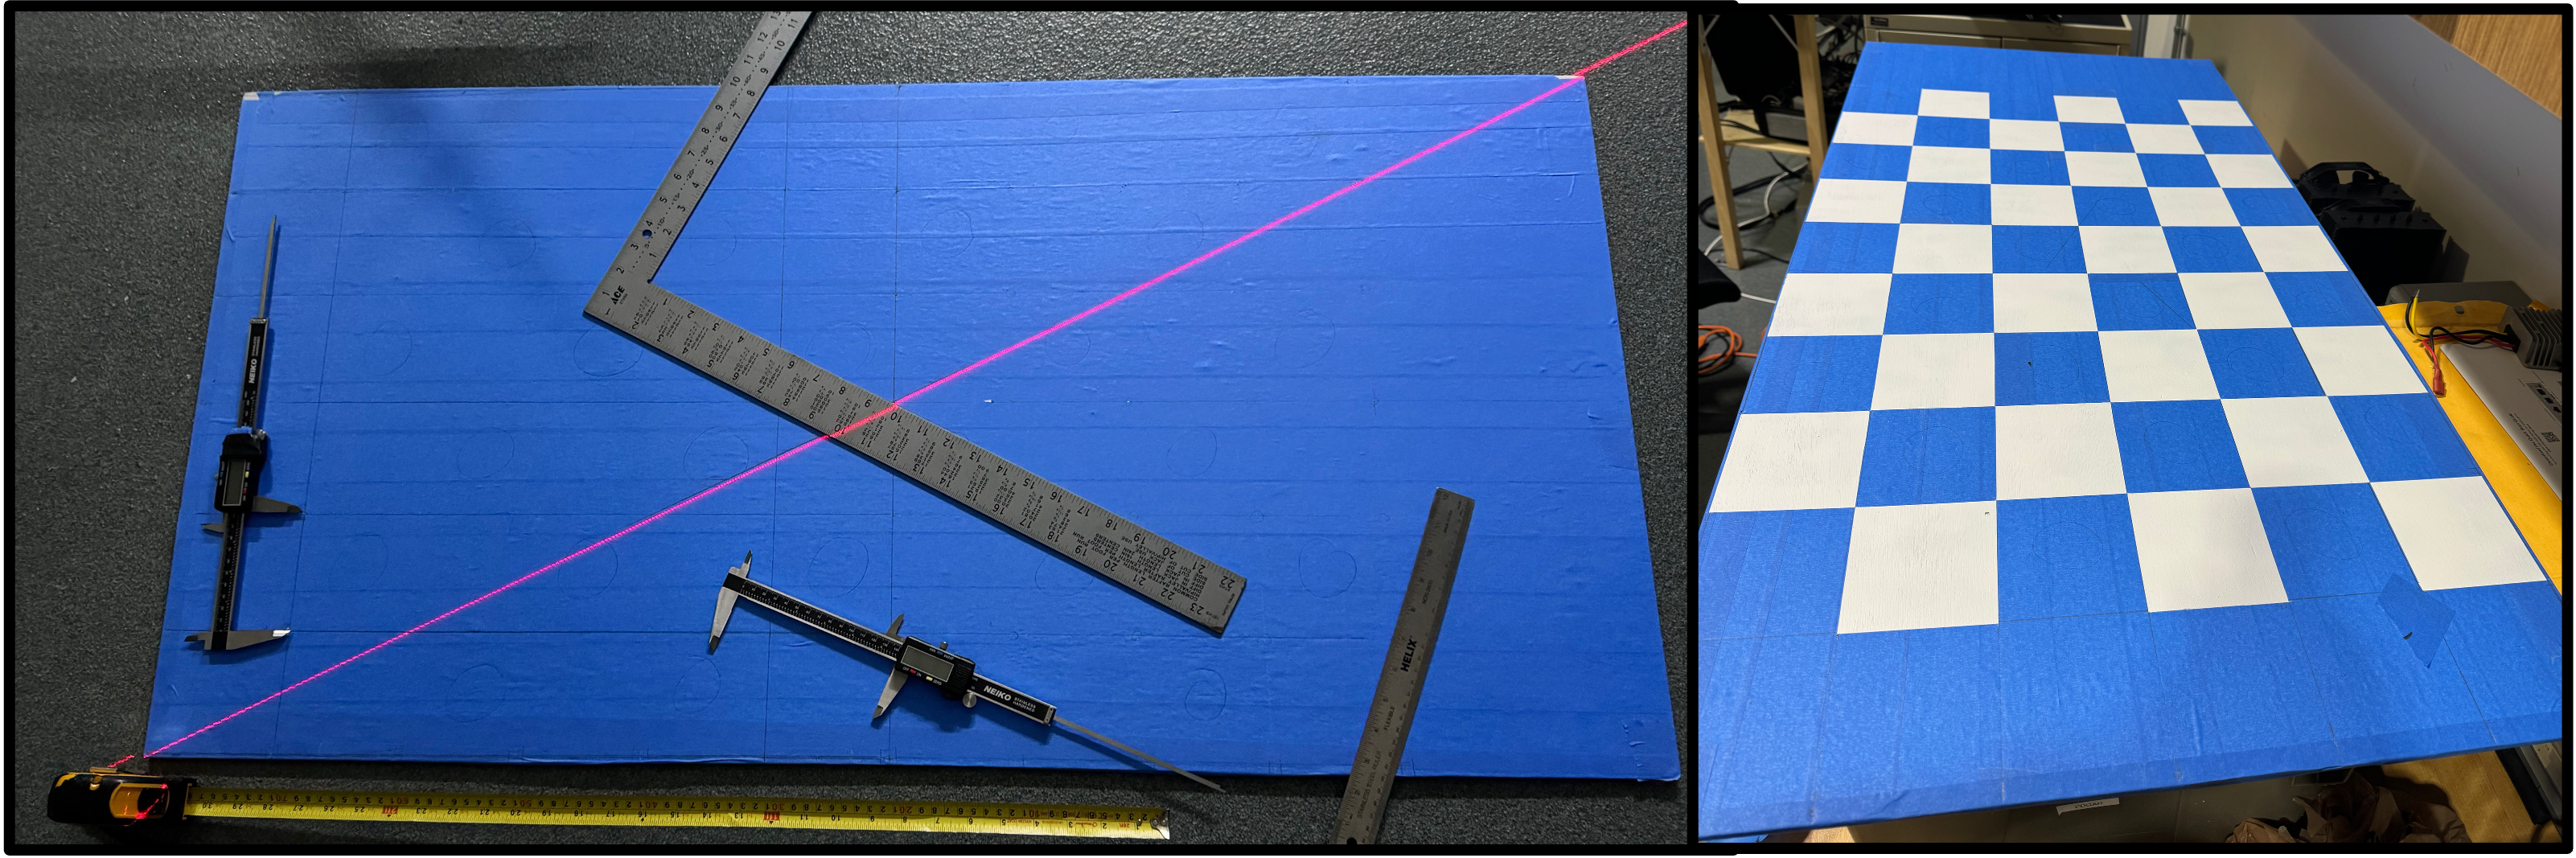
\includegraphics[width=0.9\linewidth]{Images/Checkerboard_new.png}
    \caption{New precision-painted checkerboard target used for intrinsic calibration.}
    \label{fig:checkerboard_new}
\end{figure}

\begin{figure}[htbp]
    \centering
    \includegraphics[width=0.9\linewidth]{Images/HDR_calib_error.png}
    \caption{Initial HDR camera calibration yielded a mean re-projection error of 0.63~pixels across the dataset.\textcolor{red}{reproduce graphic with larger text and landscape orientation. no need for square aspect ratio.}}
    \label{fig:HDR_calib_error}
\end{figure}

\subsubsection{Camera to LiDAR Extrinsic Calibration} \label{camLidar_calib}
\subfile{sections/camlidar_calib}

\begin{figure}[htbp]
\centering
\makebox[\textwidth][c]{
    \begin{subfigure}[t]{0.44\textwidth}
        \centering
        \includegraphics[width=\textwidth]{Images/checkerboard.png}
        \caption{Composite image of multiple checkerboard target locations.}
        \label{fig:checkerboard}
    \end{subfigure}
    \hspace{2em}
    \begin{subfigure}[t]{0.44\textwidth}
        \centering
        \includegraphics[width=\textwidth]{Images/LiDAR_calib.png}
        \caption{Composite of checkerboard locations in the LiDAR reference frame.}
        \label{fig:LiDAR_calib}
    \end{subfigure}
}
\caption{Checkerboard targets used for camera intrinsic (left) and LiDAR extrinsic (right) calibration. Red dots mark detected corner points transformed into the LiDAR frame using the initial extrinsic estimate.}
\label{fig:camLidar_calib}
\end{figure}

\subsubsection{Camera–LiDAR Calibration Results} \label{sec:camera-lidar_results}
\subfile{sections/results_camera-lidar}

\begin{figure}[htbp]
    \centering
    \includegraphics[width=0.8\linewidth]{Images/calib_checkers.png}
    \caption{Example of matched LiDAR point cloud and camera checkerboard detections used for extrinsic calibration.}
    \label{fig:calib_check}
\end{figure}

\begin{figure}[htp]
\begin{subfigure}{\textwidth}
\centering
\includegraphics[width=0.94\linewidth]{Images/LiDAR_features.png}
    \caption{}
\end{subfigure}
\bigskip
\begin{subfigure}{\textwidth}
\centering
\includegraphics[width=0.94\linewidth]{Images/LiDAR_calib_fence.png}
    \caption{}
\end{subfigure}
\caption{Vertical (red) and horizontal (green) macro-level features within the point cloud (a) are isolated (b) to support visual refinement of the camera–LiDAR alignment.}
\end{figure}

\begin{figure}[ht]
    \centering
    \includegraphics[width=0.8\linewidth]{Images/LiDAR_overlay4.png}
    \caption{Initial calibration result showing early ROI-based alignment with overlaid geometric guides for evaluation.}
    \label{fig:LiDAR_overlay4}
\end{figure}
\begin{figure}[htp]
\begin{subfigure}{\textwidth}
\centering
\includegraphics[width=0.94\linewidth]{Images/LiDAR_overlay3A.png}
    \caption{Three isolated regions of interest (ROI) in the LiDAR point cloud.}
    \label{fig:LiDAR_overlay3A}
\end{subfigure}
\bigskip
\begin{subfigure}{\textwidth}
\centering
\includegraphics[width=0.94\linewidth]{Images/LiDAR_overlay3B.png}
    \caption{}
    \label{fig:LiDAR_overlay3B.png}
\end{subfigure}
\caption{Final camera–LiDAR calibration. LiDAR ROIs containing identifiable geometry (a) are projected as red pixels onto the HDR image (b) to confirm alignment quality.}
\label{HDR_calib_final}
\end{figure}

%%%%%%%%%%%%%%%%%%%%%%%%%%%%%%%%%%%%%%%%%%%%%%%%%%%
% \subsection{Results: Spatial Calibration} \label{sec:spatial_calib_results}
% \subsubsection{LiDAR–LiDAR Calibration} \label{results_lidarLidar_calib}
% \subfile{sections/results_lidarlidar}

% \begin{figure}[ht]
% \centering
%         \includegraphics[width=0.95\textwidth]{Images/livox_viewer.png} 
% \caption{Data from port (red), center (green), and starboard (yellow) Livox Units as viewed within the Livox Viewer software (left), and the integrated calibration tool with estimated extrinsic parameters shown (right). }
% \label{fig:LidarLidar_calib}
% \end{figure}





\subsection{Temporal Calibration} \label{time_sync}
\subfile{sections/time_sync}

\subsubsection{Camera Synchronization} \label{time_sync_cam}
\subfile{sections/time_sync_cam}

\subsubsection{Network Synchronization} \label{time_sync_lan}
\subfile{sections/lan_sync}

% \subsection{Results: Temporal Synchronization} \label{results_time_sync_cam}
\subfile{sections/results_time_sync}

\section{Sensor Data and Dataset} \label{sec:sensor_data_dataset}
\subfile{sections/sensor_data}



%%%%%%%%%%%%%%%%%%%%%%%%%%%%%%%%%%%%%%%%%%%%%%%%%%%
%%%%%%%%%%%%%%%%%%%%%%%%%%%%%%%%%%%%%%%%%%%%%%%%%%%
%%%%%%%%%%%%%%%%%%%%%%%%%%%%%%%%%%%%%%%%%%%%%%%%%%%
\chapter{Real-time Object Detection} \label{realtime_object_detection}
% \subfile{sections/real_time_obj_det}
% % a brief introduction to the chapter and overview of model selection prior to method description
% % 2 to 3 paragraphs

% \section{YOLO} \label{yolo}
% \subfile{sections/yolo}
% % This section only discusses the methods used for the YOLO object detection. 
% % 3 to 4 paragraphs

% %%%%%%%%%%%%%%%%%%%%%%%%%%%%%%%%%%%%%%%%%%%%%%%%%%%%%%%%%%%%%%
% \subsection{YOLO Training Data} \label{sec:yolo_training_data}
% % \subfile{sections/training_data_yolo}






% \section{GB-CACHE} \label{gbcache}
% \subfile{sections/gbcache}
% % This section only discusses the methods used for the GB-CACHE object detection.
% % 3 to 4 paragraphs

% \subsection{GB-CACHE Training Data} \label{training_data_gbcache}
% % \subfile{sections/training_data_gbcache}

% \section{Classification Results} \label{sec:classify}
% \subfile{sections/sec:classify}

% \subsection{YOLO Performance} \label{performance_yolo}
% \subfile{sections/performance_yolo}

% \subsection{GB-CACHE Performance} \label{performance_gbcache}
% \subfile{sections/performance_gbcache}

% \subsection{Feature Relevance} \label{features_gbcache}
% \subfile{sections/features_gbcache}

% \begin{figure}
%     \centering
%     \includegraphics[width=0.95\linewidth]{Images/MI_analysis.png}
%     \caption{Caption}
%     \label{fig:MI_analysis}
% \end{figure}

% \begin{figure}
%     \centering
%     \includegraphics[width=0.95\linewidth]{Images/MI_pairwise.png}
%     \caption{Caption}
%     \label{fig:MI_pairwise}
% \end{figure}

% \section{Detection Results} \label{detect_results}
% \subfile{sections/detect_results}

% \section{Late Fusion} \label{fusion}
% \subfile{sections/fusion}
% % This section only discusses the methods used for the late fusion object detection. 

% % \section{Model Performance} \label{performance}
% % \subfile{sections/performance}
% % This section will hold all results from analysis from the YOLO, GB cache, and late fusion techniques. 



Real-time object detection lies at the core of autonomous perception, enabling vehicles to interpret their surroundings and respond safely to dynamic environments.
Effective detection requires identifying, classifying, and localizing objects rapidly enough to support decision-making and control loops, often under constraints of limited onboard computing and bandwidth.
In this work, these challenges are examined through vision and LiDAR detection pipelines implemented on the Minion sensing platform.

The central focus of this investigation is the development of a late-fusion framework that integrates information from both sensing domains to enhance detection robustness and confidence.
This framework represents the primary contribution of the research, demonstrating how visual and LiDAR detections can be combined at the decision level to leverage the complementary strengths of each sensing modality while mitigating their individual limitations.

To establish a meaningful basis for evaluation, two single-modality detection systems were selected as comparative baselines.
YOLOv8 exemplifies data-driven neural network detectors optimized for vision-based perception, and was selected for its status as one of the most widely adopted vision-based object detection methods.
GB-CACHE is a deterministic algorithm designed for LiDAR-based object detection and classification.
% Each of these models was selected for its robust nature and real-time capability, and provides contrast between neural network and deterministic-based approaches.
% ---
% These two approaches represent two distinct strategies for real-time perception, and the late-fusion method developed in this work integrates their complementary strengths to achieve higher confidence detections across a range of operating conditions.
% YOLOv8 was selected for its status as one of the most widely adopted and optimized real-time vision networks, capable of achieving high detection accuracy and efficient inference on GPU-based platforms.
% Its inclusion provides a mature and well-understood benchmark for camera-based perception, as well as a reliable reference for evaluating the complementary benefits of late fusion.
% ---
% GB-CACHE was selected as the real-time object detection method with LiDAR data. 
% This method was designed specifically for the sparse nature of maritime point clouds and performs clustering, segmentation, and classification of objects without the computational overhead or data dependency of neural network–based LiDAR methods. 
% The deterministic nature of this algorithm provides an excellent comparison to YOLO and also a robust method for late fusion, as described in Section~\ref{late_fusion}.
% This enables strict, transparent rule enforcement in clustering and segmentation, providing a level of interpretability and control not inherently available in black-box deep learning architectures.
% Its use of concave-hull extraction provides boundary representations more meaningful for maritime navigation than the simplified three-dimension bounding boxes produced by models such as PointNet or VoxelNet.
% This geometry-driven approach broadens the scope of the comparative study, especially given that the advantages of neural LiDAR methods for real-time deployment remain unproven.
% ---
Each of these models was selected for its robust, real-time capabilities and to provide a clear contrast between neural network and deterministic approaches. 
This chapter examines both models, detailing its methods, training, efficiency, detection, and classification results.
Section~\ref{yolo} presents the YOLOv8 vision-based detector and its implementation for real-time object recognition.
Section~\ref{gbcache} describes the GB-CACHE algorithm for LiDAR-based clustering and object segmentation.
Finally, this research combines the decisions from each of these detection modes in a late-fusion framework in Section~\ref{fusion} and evaluates the performance of fused results relative to the single-modality detectors through a comparative analysis of detection accuracy, computational efficiency, and real-time operation.

% These two approaches represent two distinct strategies for real-time perception, and the late-fusion method developed in this work integrates their complementary strengths to achieve higher confidence detections across a range of operating conditions.
% The following sections examine each detection method in sequence.
% Section~\ref{yolo} presents the YOLOv8 vision-based detector and its implementation for real-time object recognition.
% Section~\ref{gbcache} describes the GB-CACHE algorithm for LiDAR-based clustering and object segmentation.
% Finally, Section~\ref{fusion} introduces the late-fusion framework developed in this research and evaluates its performance relative to the single-modality detectors through a comparative analysis of detection accuracy, computational efficiency, and real-time operation.

%%%%%%%%%%%%%%%%%%%%%%%%%%%%%%%%%%%%%%%%%%%%%%%%%%%%%%%%
\section{YOLO} \label{yolo}

% Purpose and Context
The eighth generation of the \ac{YOLO} framework was selected to provide a baseline performance for real-time vision-based detection in this research. 
This method of detection gained popularity for its ease of use and implementation for detecting and localizing objects within an image.
Once an object is detected, the pixel coordinates it occupies within the image frame are bounded with a rectangle known as the bounding box (see Figure \ref{fig:YOLO_tower}).
Its open-source models are pretrained on the COCO dataset, a large repository containing approximately 1.5 million labeled images, and are provided in various sizes and qualities, which can be deployed on a wide variety of edge computing hardware.
Additionally, transfer learning is simple to apply, allowing these models to be tailored for more specific use cases, such as maritime environments.

\begin{figure}
    \centering
    \includegraphics[width=0.75\linewidth]{Images/YOLO_ex1.png}
    \caption{Rectangular bounding boxes placed around maritime objects detected by a re-trained YOLO detection model.}
    \label{fig:YOLO_tower}
\end{figure}

The name YOLO refers to the single-shot convolutional neural network architecture used to perform both detection and localization in a single pass.
While this design was key to achieving real-time detection speeds, the accuracy of an object’s bounding box within an image was limited by the available training data. 
Prior to the release of version 8 in 2023, the model required that the center and bounds of each detected object be explicitly encoded within the model, requiring a large corpus of labeled data for training.
Version 8 introduced dual detection heads at the end of the CNN architecture: the first head identifies if and where an object is present within the image, while the second head determines the object's bounding box.
This “anchor-free” architectural change not only improves the reliability of object localization but also reduces the burden of transfer learning required for fine-tuning pre-trained models in earlier versions\cite{ultralytics}.

The widespread adoption and speed of YOLOv8 make it the optimal choice for providing a baseline visual detection method, and the fundamental architectural changes in this version validate its selection for a late-fusion approach.
% However, this mode of detection is not without its compromises, \textcolor{red}{as will be detailed in Section ____.}



% The YOLO Framework
% Describe the principle succinctly:

% YOLOv8 Architecture
% This section should flow from general framework to version-specific improvements:

% Image Resolution and Input Scaling
% Transition to operational detail and experimental consistency:

% Detection Scale and Spatial Sensitivity
% Discuss how feature maps relate to the detection limit:

% Model Constraints and Applicability
% Then note practical limitations and their relevance:

% Implications for Real-Time Fusion
% Conclude the section by connecting to your larger research goal:

% \textcolor{red}{To establish a performance baseline for real-time, vision-based object detection, this study employed the You Only Look Once (YOLO) framework, a single-stage convolutional neural network (CNN) architecture designed for end-to-end detection and classification. Unlike two-stage detectors that separately generate region proposals before classification, YOLO formulates detection as a direct regression problem, predicting bounding box coordinates and class probabilities simultaneously. This design allows all detections to occur in a single computational pass, providing the speed necessary for autonomous and embedded sensing applications. The visual detection results presented here serve as the reference modality for comparison with LiDAR-based detection methods and for evaluating computational performance in the subsequent late-fusion framework.}

% \textcolor{red}{
% The eighth-generation YOLOv8 model developed by Ultralytics was selected due to its stability, active development, and high inference efficiency on modern hardware. YOLOv8 integrates several architectural refinements that enhance accuracy and convergence speed relative to previous versions. The model employs an anchor-free detection strategy, eliminating the predefined bounding-box templates that characterized earlier YOLO iterations. Instead, YOLOv8 predicts the object center, width, and height directly, simplifying configuration and improving adaptability to objects of varying aspect ratios and scales. A decoupled detection head separates the regression and classification branches of the network, allowing independent optimization of spatial and semantic components during training. The backbone of the network uses C2f (Cross-Stage Partial Fusion) modules, which improve feature reuse and gradient flow while reducing overall computation. These modifications collectively contribute to higher accuracy and reduced latency, both of which are critical for on-board real-time inference
% The model employs modern loss functions to enhance bounding-box precision. The Complete-IoU (CIoU) loss function refines localization by incorporating geometric distance and aspect ratio penalties, while the Distribution-Focal Loss (DFL) improves boundary regression stability. Together, these losses improve the correspondence between predicted and ground-truth boxes and facilitate more consistent convergence during training. The network was implemented in PyTorch using the native Ultralytics framework, which provides integrated preprocessing, data augmentation, and export utilities. This implementation enables consistent deployment across GPU-based and embedded computing platforms without manual configuration
% }
% \textcolor{red}{
% All input frames were processed at a resolution of 640 × 640 pixels, which corresponds to YOLOv8’s default operational size and the native output of the experimental imaging system. Maintaining this native resolution avoided unnecessary interpolation and ensured a one-to-one correspondence between camera pixels and network input. YOLOv8 performs detection at three spatial scales, corresponding to feature-map strides of 8, 16, and 32 pixels relative to the input. These scales allow simultaneous sensitivity to small, medium, and large objects within a single inference pass. For a 640 × 640 input image, these feature maps have effective dimensions of 80 × 80, 40 × 40, and 20 × 20 cells, respectively. Each cell in the smallest-stride feature map represents an 8 × 8 pixel region of the input image.}
% \textcolor{red}{
% Because of this multi-scale design, the network’s minimum detectable object size is bounded by the stride of the smallest feature map. Objects must occupy multiple adjacent cells to generate distinct activations; those confined to a single cell are typically lost through downsampling or non-maximal suppression. Empirical evaluation and prior literature indicate that YOLOv8 reliably detects objects approximately 16–32 pixels in width or height—roughly 0.5–1 percent of the frame area for a 640 × 640 input. Objects smaller than this threshold generally produce low-confidence or unstable detections.}
% \textcolor{red}{
% This limitation arises from several interrelated factors. First, downsampling loss in convolutional and pooling layers reduces high-frequency detail, causing very small features to disappear from deeper network layers. Second, the receptive field of later layers covers large portions of the input image, diminishing the spatial specificity required for fine-scale detections. Third, training bias inherent to datasets such as COCO and VOC, which contain relatively large annotated objects, restricts the network’s learned sensitivity to sub-pixel features. These factors collectively define the lower bound of object detectability in standard YOLOv8 configurations.}
% \textcolor{red}{
% The 640 × 640 camera used in this study matches the network’s native input dimension, permitting direct inference without rescaling and ensuring consistent timing measurements for real-time operation. This configuration provides an accurate representation of YOLOv8’s performance under embedded deployment conditions and serves as a visual-only detection baseline against which LiDAR-based methods and fused detection results are compared in later sections. The analysis presented here therefore defines the temporal and computational characteristics of the visual detection pipeline that underpin the late-fusion approach adopted in this research.
% }


%%%%%%%%%%%%%%%%%%%%%%%%%%%%%%%%%%%%%%%%%%%%%%%%%%%%%%%%
\subsection{Training Data} \label{sec:yolo_training_data}

A manually labeled image dataset was constructed to support the transfer learning and evaluation of the YOLO object detection network. 
All YOLO training images were obtained from video frames that are not present within the rosbag data.
Due to the rate of data accumulated within each rosbag described in section~\ref{sec:data_overview}, this data was recorded strategically,  whereas the cameras operated and streamed continuously.
This ensured that a large pool of video data remained separate from the main dataset and available for YOLO training.

The complete dataset contained 778 annotated images with a total of 1934 labeled maritime objects from the six classes defined in Table \ref{tab:class_map} 
Each annotation was produced through a manual labeling process for objects present within each 2880 $\times$ 860 frame. 

For this research, YOLOv8 was trained on a custom maritime dataset derived from sensor recordings collected aboard the Minion platform.
The dataset includes labeled examples of navigation markers, buoys, vessels, and other relevant maritime objects.
The final dataset contained 778 annotated images and 1934 labeled maritime objects. 
Data were divided into training, validation, and test subsets following a 70:20:10 ratio.
Each subset preserved the relative class proportions observed in the complete dataset, which contained an average of 2.5 labeled objects per image across the five categories listed in Table~\ref{tab:class_map}.
The A2 and A3 buoy variants are virtually identical when viewed in isolation, as their size difference can only be inferred through comparison or with additional depth information in the image frame. 
Because YOLO operates purely on two-dimensional image data without access to spatial depth cues, there was no practical benefit to treating these as separate classes; both were therefore labeled collectively as \texttt{round\_buoy}.
% \textcolor{blue}{Based on field observations, it is likely that A2 buoys were predominantly red, green, or blue, whereas A3 and larger buoys appeared black. 
% However, since visually similar large black buoys were also observed throughout the rosbag dataset without verified size information, these classes were merged to maintain labeling consistency.}

% \begin{table}[htbp]
% \centering
% \begin{tabular}{lccccccc}
% \hline
% Subset & Images & Labels & Tall Buoy & Round Buoy & Light Tower & Jon Boat & Sailboat \\
% \hline
% Train & 543 & 1,343 & 12.0\% & 1.4\% & 11.2\% & 15.8\% & 59.6\% \\
% Validation & 158 & 390 & 14.1\% & 1.3\% & 13.1\% & 12.8\% & 58.7\% \\
% Test & 77 & 201 & 16.4\% & 1.5\% & 9.5\% & 12.4\% & 59.7\% \\
% \hline
% Total & 778 & 1,934 &  &  &  &  &  \\
% \hline
% \end{tabular}
% \caption{YOLO dataset composition and class distribution across training, validation, and test subsets.}
% % \label{table:yolo_data_split}
% \end{table}

\begin{table}[htbp]
\centering
\begin{tabular}{lcccc}
\hline
& Train & Validation & Test & Total \\
\hline

Tall Buoy & 12.0\% & 14.1\% & 16.4\% &  \\
Round Buoy & 1.4\% & 1.3\% & 1.5\% &  \\
Light Tower & 11.2\% & 13.1\% & 9.5\% &  \\
Jon Boat & 15.8\% & 12.8\% & 12.4\% &  \\
Sailboat & 59.6\% & 58.7\% & 59.7\% &  \\
\hline
Images & 543 & 158 & 77 & 778 \\
Labels & 1,343 & 390 & 201 & 1,934 \\
\hline
\end{tabular}
\caption{YOLO dataset composition and class distribution across training, validation, and test subsets.}
\label{table:yolo_data_split}
\end{table}

% \noindent The relative consistency across all three subsets demonstrates that the temporal stratification preserved real-world object frequency while maintaining balance for training and evaluation. 
% The test set was reserved exclusively for the final performance assessment described in Chapter~\ref{realtime_object_detection}.

% \noindent Transfer learning was employed by initializing the network with weights pre-trained on a general-purpose dataset, then fine-tuning on the maritime-specific data to adapt the model to the target domain.
Fine-tuning was conducted using the Ultralytics YOLOv8 framework. \cite{ultralytics} %, employing a combination of data augmentation techniques—including random horizontal flips, exposure shifts, and image rotations—to improve robustness under varying lighting and sea-state conditions.
% Hyperparameters such as learning rate, batch size, and the number of epochs were optimized empirically to achieve stable convergence while minimizing overfitting.
To assess the tradeoff between detection accuracy and inference speed, three YOLOv8 model size variants —nano (YOLOv8n), small (YOLOv8s), and medium (YOLOv8m) were trained using the default parameters and evaluated over a set of training epochs.
Each model’s number of trainable parameters, summarized in Table~\ref{tab:yolo_variants}, corresponds to differences in backbone depth and channel width that balance model capacity against computational efficiency.
This means that smaller models can perform faster and with fewer computational resources, but will likely not achieve the same levels of performance as a larger model with more parameters.
Training was performed over a range of epochs to identify the most efficient configuration for the dataset.

The medium-sized model (YOLOv8m) exhibited no measurable improvement in mean average precision compared to the small model (YOLOv8s), while containing more than twice the parameters and only processing image frames at $\approx 74\%$ the speed of the small model.
The YOLOv8s model achieved full convergence within approximately 80 epochs without signs of overtraining and was therefore selected for subsequent testing and deployment.
The precision, recall, and other performance metrics for each model's training are provided over 100 epochs in Appendix~\ref{append_yolo}.

\begin{table}[htbp]
\centering
\begin{tabular}{l c c c c}
\hline
Model & Params (M) & FPS (RTX 3090) & mAP@50 \\
\hline
YOLOv8n & 3.2 &  110 & 0.79 \\
YOLOv8s & 11.2 &  85 & 0.84 \\
YOLOv8m & 25.9 &  63 & 0.87 \\
\hline
\end{tabular}
\caption{YOLOv8 model size comparison and mAP scores after 100 epochs.}
\label{tab:yolo_variants}
\end{table}

Each labeled image required 60 seconds to manually label (mean), and an additional 45 minutes was required for the YOLOv8-s model to converge on the dataset. 
This results in an estimated total aggregate time of 13 hours to prepare this dataset. 
% An additional 45 minutes was required

Inference timing was recorded using per-process timers to isolate image capture, pre-processing, neural inference, and post-processing durations.
This timing-based comparison allows fair assessment against non-GPU LiDAR pipelines in later sections.

\begin{figure}[htbp]
    \centering
    \includegraphics[width=0.85\linewidth]{Images/yolo/YOLO_training.png}
    \caption{YOLOv8 transfer learning convergence showing loss and mean Average Precision (mAP) trends over 80 epochs with the small model.}
    \label{fig:yolo_training_curve}
\end{figure}



\subsection{Results} \label{sec:yolo_results}

The fine-tuned YOLOv8-s model achieved the best balance of accuracy and speed for maritime operations.
Model evaluation was performed using a holdout dataset collected under variable illumination and sea states.
Performance metrics include mean Average Precision (mAP@50), precision-recall curves, and confusion matrices for key object classes such as vessels, buoys, and docks.

\begin{figure}[htbp]
    \centering
    \includegraphics[width=0.8\linewidth]{Images/yolo/YOLO_training_results.png}
    \caption{Confusion matrix for YOLOv8-s model evaluated on the test dataset.}
    \label{fig:yolo_confusion_matrix}
\end{figure}

% \begin{figure}[htbp]
%     \centering
%     \includegraphics[width=0.8\linewidth]{Images/yolo_pr_curve.png}
%     \caption{Precision–recall curve for primary object classes.}
%     \label{fig:yolo_pr_curve}
% \end{figure}

% Results indicate consistent detection performance across lighting conditions with minimal false positives on horizon clutter.
% Retraining improved small-object detection by approximately X\% compared to baseline COCO-trained weights, confirming the benefit of domain adaptation for maritime imagery.

The fine-tuned YOLOv8 network serves as the visual baseline for comparison with LiDAR-based object detection methods presented in Section~\ref{gbcache}.
By isolating timing metrics for each processing stage, the performance comparison remains hardware-agnostic.
This approach emphasizes algorithmic latency, rather than total frame rate, as the primary metric for evaluating real-time feasibility in multi-sensor fusion.

%%%%%%%%%%%%%%%%%%%%%%%%%%%%%%%%%%%%%%%%%%%%%%%%%%%%%%%%
\section{GB-CACHE} \label{gbcache}
%\subfile{sections/gbcache}

Grid-Based Clustered Adaptive Concave Hull Extraction (GB-CACHE) is a spatial indexing and clustering methodology specifically designed for efficient processing of three-dimensional point cloud data in maritime environments. 
The algorithm provides rapid object segmentation through grid-based spatial partitioning followed by concave hull boundary extraction, enabling the real-time detection performance essential for autonomous navigation safety.

\subsection{Grid-Based Spatial Indexing and Clustering} \label{gbcache_clustering}
% ### Grid-Based Spatial Indexing and Clustering

The fundamental principle underlying GB-CACHE involves partitioning the three-dimensional LiDAR point cloud into a regular grid structure that facilitates efficient spatial queries and proximity-based clustering. Rather than evaluating pairwise distances among all points, the grid-based approach achieves linear complexity by organizing points into fixed spatial bins. Each grid cell represents a discrete volumetric region, and points falling within the same cell or adjacent cells are considered spatially proximate.
This spatial indexing approach proves particularly advantageous for maritime LiDAR data. 
% The majority of returns originate from discrete floating objects rather than continuous surfaces, and the predominantly planar water surface produces minimal returns. 
The sparse nature of maritime point clouds enables the grid structure to efficiently isolate regions containing potential objects while discarding empty space, thereby reducing both memory consumption and computational overhead.

% Once the point cloud is organized spatially, connected component analysis identifies clusters of occupied grid cells representing distinct physical objects. 
% The clustering operation employs 26-connectivity criteria (vertex-connected), grouping cells that share faces, edges, or vertices. 
% This connectivity threshold preserves object integrity for maritime targets that may exhibit irregular geometric configurations, particularly navigation buoys with narrow mounting hardware or vessels with complex superstructures. 
% Following initial clustering, size-based filtering removes clusters that are inconsistent with the target object dimensions, thereby eliminating obvious false positives before feature extraction.

% ### Concave Hull Extraction and Feature Calculation
\subsection{Concave Hull and Feature Extraction} \label{gbcache_features}

For each cluster identified through the grid-based segmentation, GB-CACHE extracts a concave hull boundary that defines the object's spatial extent. 
While convex hulls guarantee computational efficiency and provide simple bounding representations, concave hulls more accurately capture object shape by allowing inward boundary curvature. 
This distinction proves critical for maritime objects with non-convex geometries, including U-shaped channel markers or vessels with significant superstructure features.

The concave hull generation process balances boundary accuracy against computational cost through a configurable complexity parameter that controls the degree of boundary concavity. 
The resulting polygon provides a compact geometric representation suitable for both visualization and feature extraction for subsequent classification. 
Beyond simple bounding boxes, concave hull boundaries enable the calculation of geometric features, such as area and perimeter, that support object classification. 

The algorithmic design prioritizes computational efficiency to enable real-time processing on autonomous surface vessel hardware with limited computing resources. 
The processing pipeline operates incrementally on each LiDAR scan, maintaining no temporal history and requiring no iterative refinement. 
This stateless design simplifies implementation and guarantees bounded worst-case execution time, a critical property for safety-critical autonomous systems. 
Memory requirements scale with grid dimensions rather than point count, providing predictable resource consumption independent of scene complexity.


% \begin{figure}[htpb]
%     \centering
%     \includegraphics[width=0.95\linewidth]{Images/gbcache/gbcache_flow.png}
%     \caption{A block diagram of GB-CACHE process flow. Clock colors correspond to measured segments of the GB-CACHE process: Ground Plane Removal (blue), Add Points (lime green), and clustering/Convex Hull Extraction/Classification (teal).}
%     \label{fig:gbcache_flow}
% \end{figure}



% \begin{figure}
%     \centering
%     \includegraphics[width=0.95\linewidth]{Images/gbcache_flow.png}
%     \caption{Rectangular bounding boxes placed around maritime objects detected by a re-trained YOLO detection model.}
%     \label{fig:gbcache_flow}
% \end{figure}


% \begin{figure}
%     \centering
%     \includegraphics[width=0.5\linewidth]{Images/gbcache_flow.png}
%     \caption{Functional block diagram of the GB-CACHE workflow.}
%     \label{fig:gbcache_flow}
% \end{figure}


% \begin{table}[htbp]
% \centering
% \begin{tabular}{lll}
% \hline
% \multicolumn{3}{c}{GB-CACHE: Object Classification Features}\\
% \hline
% \hline
% \textbf{No.} & \textbf{Feature Type} & \textbf{Description} \\ 
% \hline
% 1 & Maximum Intensity & Peak LiDAR return intensity \\
% 2 & Minimum Intensity & Lowest LiDAR return intensity \\
% 3 & Average Intensity & Mean LiDAR return intensity \\
% 4 & Intensity Standard Deviation & Variation in return intensity \\
% 5 & Maximum Height & Vertical extent of the object \\
% 6 & Filled Cell Count & Number of occupied grid cells \\
% 7 & Polygon Perimeter & Boundary length of concave hull \\
% 8 & Polygon Area & Enclosed area of concave hull \\
% 9 & 2D Minor Axis Length & Shorter principal axis of object shape \\
% 10 & 2D Major Axis Length & Longer principal axis of object shape \\
% \hline
% \end{tabular}
% \caption{Features used for GB-CACHE multivariate classification.}
% \label{tab:gbcache_features}
% \end{table}

% \begin{figure}[htbp]
%     \centering
%     \includegraphics[width=0.95\linewidth]{Images/info_theory_chart_1.png}
%     \caption{Caption}
%     \label{fig:infoTheory_chartsA}
% \end{figure}

% \begin{figure}[htbp]
%     \centering
%     \includegraphics[width=0.8\linewidth]{Images/info_theory_chart_2.png}
%     \caption{Caption}
%     \label{fig:infoTheory_charts}
% \end{figure}

%%%%%%%%%%%%%%%%%%%%%%%%%%%%%%%%%%%%%%%%%%%%%%%%%%%%%%%%
\subsection{Training Data} \label{training_data_gbcache}

Training data for the GB-CACHE's MGC was obtained from data within the rosbag dataset described in Section~\ref{sec:data_overview}.

In general, each class of object was observed in a stationary position at a range of 40 to 60 meters as the Minion \ac{USV} approached the object to a range of 5 meters. 
In total, this results in approximately 20 to 30 seconds of training data for each object class.
The only notable exception to this method is for the Jon boat class. 
Due to constraints on available time for data collection, training data for this class consisted of Minion remaining stationary, and the Jon boat approaching the \ac{USV} from a similar range and rate.
At least one rosbag within the dataset was recorded for training each of the six object classes, and these bag IDs are listed in Table \textcolor{red}{insert table}.

The training bagfiles are post-processed with MATLAB to extract the target object ID and metadata from the \texttt{obj\_w\_class} topic over the identified time period.
This metadata is processed to extract 10 features used for classification, which are provided in Table~\ref{tab:gbcache_features}.

\begin{table}[htpb]
\centering
\begin{tabular}{cc}
\hline
Class Label & No. Samples \\
\hline
\hline
Tall Buoy   & 4342        \\
A2 Buoy     & 861         \\
A3 Buoy     & 979         \\
Light Tower & 1197        \\
Jon Boat    & 1502        \\
Sailboat    & 2103       \\
\hline
\end{tabular}
\caption{Number of samples utilized to train the multivariate Gaussian classifier.}
\end{table}

The post-processing of LiDAR data requires live playback of the bag file. 
Each sample is processed at a rate of 5 Hz, resulting in a total of 36.6 minutes for data labeling.
Splitting the data into training and test sets only takes two to three minutes per class, and training is completed within a matter of seconds.
The total time required to collect and train this classifier method for all six classes is less than an hour.

Training is performed by examining the ten features in each of the training samples. 
From this data, a coefficient, mean vector, and covariance matrix are determined for all ten features. 
This information is saved into separate files for each class and loaded into ROS at runtime.

The results of the MGC classification training show 97.49\% accuracy, with a breakdown of each class provided in Figure~\ref{livox_train}

\begin{figure}
    \centering
    \includegraphics[width=0.5\linewidth]{Images/livox_train.png}
    \caption{Training accuracy for the multivariate Gaussian classifier across each of the six maritime object classes}
    \label{livox_train}
\end{figure}

Rosbags from which LiDAR training data was collected are not included in the final testing set used to provide analysis on detection results.

\subsection{Results} \label{sec:gbcache_results}

To evaluate computational performance, the GB-CACHE processing sequence is grouped into three subroutines.
These subroutines correspond to the sequential stages that handle LiDAR data input, spatial filtering, and map updating during each processing cycle.
The first subroutine, "Filter Points," removes points reflected from the water's surface, reducing noise and false positives with object detection.
The second routine, "Add Points," assigns the remaining raw LiDAR returns to the occupancy grid, \textcolor{blue}{listing them as unprocessed}.
The final subroutine, "Map Points", combines segmentation, clustering, and classification.
Figure~\ref{fig:gbcache_flow_analysis} provides a block diagram of the GB-CACHE workflow with these three subroutines windowing the related tasks.

---

Each rosbag was replayed on the same Minion PC hardware that recorded it, providing only the raw LiDAR data and navigational topics to the GB-CACHE ROS node. 
This approach perfectly simulates the operational data processing environment. 
The execution time of each subroutine was measured along with the number of points processed by each function. 
Overall, more than 1.7 million executions of "Filter Points" and "Add Points" and more than 45 thousand executions of "Update Map" were measured across the entire dataset.

The LiDAR data is transmitted at a rate of 100 Hz from three Livox Horizon units, while the output ROS topic \texttt{Obj\_w\_class} that this algorithm generates is published at 5 Hz. 
The first two subroutines examined, "Filter Points" and "Add Points", execute sequentially without parallelization. 
These processes must handle raw data from all three LiDAR units at 100 Hz; therefore, these two subroutines must execute at least once every 3.33 milliseconds. 
The "Update Map" subroutine receives the output of the first two, but only outputs detections at 5 Hz, providing an allotted execution time of 200 milliseconds per cycle.



\begin{figure}
    \centering
    \includegraphics[width=0.95\linewidth]{Images/gbcache_flow.png}
    \caption{The three main portions of the GB-CACHE process which were examined for performance}
    \label{fig:gbcache_flow_analysis}
\end{figure}


\begin{table}[htbp]
\centering
\begin{tabular}{lccccc}
\hline
Subroutine & Samples & Avg Duration (ms) & Allotted Time (ms) & \% of Allotted Time\\
\hline
Filter Points & 1,701,153 & 0.009 &  3.33 & 0.26 \% \\
Add Points & 1,701,153 & 0.140 &  3.33 & 4.21 \% \\
Update Map & 45,746 & 8.002 & 200 & 4.00 \% \\
\hline
\end{tabular}
\caption{Average execution time and percentage of allotted processing time for each GB-CACHE subroutine.}
\label{tbl:gbcache_subroutine_results}
\end{table}

% timing analysis
Performance analysis of the GB-CACHE implementation on the Minion platform demonstrates exceptional computational efficiency compatible with real-time autonomous navigation requirements. 
The combined point-processing stages execute well within the available time budget. 

The data shown in table~\ref{tbl:gbcache_subroutine_results} indicate that GB-CACHE's computational performance is dominated by the segmentation and classification phase. 
Yet, this process remains well below the latency threshold required for real-time operation, and the preceding "Filter Points" and "Add Points" steps contribute negligibly to the total cycle time. 

The Filter Points and Add Points subroutines were measured to have a combined mean execution time of  0.149 ms per cycle, which corresponds to approximately 4.5\% of the 3.33 ms processing window allocated for LiDAR data processing. 
This indicates that online point filtering and insertion impose minimal computational load relative to the cycle time.
% \textcolor{blue}{need more discussion here of capability and comp head-room. Also discuss the plateau of filterpts and clustering of acquirePts scatter plots}

In comparison, the Update Map subroutine requires an average of 8.002 ms per update, utilizing only about 4.0\% of its 200 ms allocation. 
All three stages, therefore, maintain substantial timing margins, confirming that the mapping pipeline can operate in real time without approaching its latency constraints. 
Histograms of the execution times for each subroutine are provided along with normalized scatter plots of execution time against the number of points processed in Figures~\ref{fig:gbcache_filter_points}, \ref{fig:gbcache_add_points}, and \ref{fig:gbcache_update_map}.

The data shown in table~\ref{tbl:gbcache_subroutine_results} indicate that GB-CACHE's computational performance is dominated by the segmentation and classification phase. 
Yet, this process remains well below the latency threshold required for real-time operation, and the preceding "Filter Points" and "Add Points" steps contribute negligibly to the total cycle time. 


% timing/points analysis
The scatter plots of Figures~\ref{fig:gbcache_filter_points}, \ref{fig:gbcache_add_points}, and \ref{fig:gbcache_update_map} reveal essential information regarding how well the method can scale. 
The scatter plots 
Plotting each execution time against the number of points processed reveals how the algorithm scales computationally. 
% \textcolor{red}{"Filter Points" looks to appear to have a linear histogram, with an upper bound to the number of points returned most frequently. "Add Points" looks to have a near-linear to somewhat logarithmic scaling.}
% The grid representation compresses sparse maritime point clouds into compact occupancy structures, reducing memory bandwidth requirements compared to maintaining full point coordinates. 
% This compression proves particularly advantageous for maritime environments where objects occupy a small fraction of the sensor's field of view.

% subfigures \ref{fig:gbcache_update_map} (b) and \ref{fig:gbcache_update_map} (c) vary slightly to Figures~\ref{fig:gbcache_filter_points}, \ref{fig:gbcache_add_points}.
Figures~\ref{fig:gbcache_filter_points}, \ref{fig:gbcache_add_points}, and \ref{fig:gbcache_update_map}, provide a histogram of the execution times measured for each of the subroutines. This data is also provided in scatter plots as a function of the number of points processed in figures~\ref{fig:gbcache_filter_points} and\ref{fig:gbcache_add_points}, and as a function of object perimeter length in \ref{fig:gbcache_update_map} (b) and object surface area in \ref{fig:gbcache_update_map} (c).


\ref{fig:gbcache_update_map} and \ref{fig:gbcache_update_map} (c) vary slightly to 
Rather than plotting the execution of the "Update Map" subroutine against the number of points, we examined the duration as a function of the mean length and mean area of observed objects. 
The data shows a strong linear correlation with object perimeter length and a similarly strong quadratic relationship with object area. 
This predictable scaling behavior enables the reliable estimation of worst-case execution time for safety-critical autonomous systems. It suggests potential algorithmic improvements to optimize how shorelines are handled when they appear within the LiDAR return data.
% This is of particular interest for maritime operations in littoral zones, suggesting potential algorithmic improvements to optimize how shorelines are handled when they appear within the LiDAR return data.


% The "Update Map" operation, while more computationally intensive than the filtering stages, exhibits strong linear correlation with object geometric complexity—specifically, polygon perimeter and surface area. 
% This predictable scaling behavior enables the reliable estimation of worst-case execution time for safety-critical autonomous systems. 


% hardware analysis
% \textcolor{red}{Hardware resource utilization remains minimal during typical operation, with both processor and memory consumption well below capacity thresholds, providing substantial computational headroom for concurrent navigation and control processes.}



\begin{figure}[htbp]
\centering
\makebox[\textwidth][c]{
    \begin{subfigure}[t]{0.44\textwidth}
        \centering
        \includegraphics[width=\textwidth]{Images/gbcache/filter_points_scatter.png}
        \caption{Scatter plot of duration of \texttt{filter\_points} against number of LiDAR points}
        \label{fig:gbcache_filter_points_scatter}
    \end{subfigure}
    \hspace{2em} % horizontal spacing between them
    \begin{subfigure}[t]{0.44\textwidth}
        \centering
        \includegraphics[width=\textwidth]{Images/gbcache/filter_points_hist.png}
        \caption{Histogram of duration of \texttt{filter\_points} against number of LiDAR points}
        \label{fig:gbcache_filter_points_hist}
    \end{subfigure}
}
\caption{Scatter (a) and histogram (b) plots of \texttt{filter\_points} process plotted against number of LiDAR points}
\label{fig:gbcache_filter_points}
\end{figure}

\begin{figure}[htbp]
\centering
\makebox[\textwidth][c]{
    \begin{subfigure}[t]{0.44\textwidth}
        \centering
        \includegraphics[width=\textwidth]{Images/gbcache/Add_points_scatter.png}
        \caption{Scatter plot of duration of \texttt{add\_points} against number of LiDAR points}
        \label{fig:gbcache_add_points_scatter}
    \end{subfigure}
    \hspace{2em} % horizontal spacing between them
    \begin{subfigure}[t]{0.44\textwidth}
        \centering
        \includegraphics[width=\textwidth]{Images/gbcache/Add_points_hist.png}
        \caption{Histogram of duration of \texttt{add\_points} against number of LiDAR points}
        \label{fig:gbcache_add_points_hist}
    \end{subfigure}
}
\caption{Scatter (a) and histogram (b) plots of \texttt{add\_points} process plotted against number of LiDAR points}
\label{fig:gbcache_add_points}
\end{figure}

\begin{figure}[htbp]
    \centering
    % Subfigure (a)
    \begin{subfigure}[b]{0.44\linewidth}
        \centering
        \includegraphics[width=\linewidth]{Images/gbcache/Update_Map_hist.png}
        \caption{Histogram of duration of \texttt{map\_update} against number of LiDAR points}
        \label{fig:gbcache_update_map_hist}
    \end{subfigure}
    \vspace{1em} % vertical spacing between subfigures
    % Subfigure (b)
    \begin{subfigure}[b]{0.8\linewidth}
        \centering
        \includegraphics[width=\linewidth]{Images/gbcache/Update_Map_scatter.png}
        \caption{Two scatter plots of duration of \texttt{map\_update} against average perimeter length of polygon (left), and against average area of polygon (right). The line of best-fit is shown in red for each, with associated polynomial values of: $x^2 = -0.0727, x^1 = -0.0151, x^0 = -0.0151$ (left) and $x^2 = 0.2556, x^1 = -0.00913, x^0 = -0.00913$ (right)}.
        \label{fig:gbcache_update_map_scatter}
    \end{subfigure}

    \caption{Histogram of \texttt{map\_update} execution duration (a) and scatter plots (b) of execution time plotted as a function of detected object perimeter (left) and object surface area (right) number of LiDAR points}
    \label{fig:gbcache_update_map}
\end{figure}



%%%%%%%%%%%%%%%%%%%%%%%%%%%%%%%%%%%%%%%%%%%%%%%%%%%%%%%%
\subsection{MGC Feature Analysis} \label{features_gbcache}
% \subsubsection{GB-CACHE Features} 

% \subsection{Multivariate Gaussian Classifier} \label{gbcache_mgc}
% A multivariate Gaussian classifier was selected to be paired with GB-CACHE for object classification. 
% Research performed by Thompson \cite{thompson2017} previously determined this classification method as superior to classification with support vector machines, though no investigation has been performed to examine the effectiveness of the set of ten features used.

The classification of objects utilizes a Multivariate Gaussian Classifier (MGC) framework to model the joint probability distribution of extracted features for each object class. 
Under the assumption that features follow multivariate Gaussian distributions within each class, the classifier computes class likelihoods using covariance matrices and mean vectors estimated from labeled training data. 
This approach offers computational efficiency during inference while capturing correlations among features, thereby enhancing discriminative power.

% The Gaussian assumption simplifies the classification problem to estimating a probability density function for each class from the feature distributions within the training samples and applying Bayes' rule during inference to select the most probable class. 
% For a feature vector representing an observed object, the classifier evaluates the probability density under each class-specific Gaussian model and assigns the class yielding maximum posterior probability. 
% This framework naturally accommodates multiple object classes and provides confidence estimates through the posterior probability values.
The Gaussian assumption simplifies the classification problem to estimating a probability density function for each class from the feature distributions within the training samples and applying Bayes' rule during inference to select the most probable class.
This framework naturally accommodates multiple object classes and provides confidence estimates through the posterior probability values.



Ten features are extracted in total.  
Four intensity features are identified from the raw, segmented LiDAR data, and six additional features are derived from the extracted concave hull geometry.
These ten features are listed with a brief description in Table~\ref{tab:gbcache_features}.
While Thompson \cite{thompson2017} demonstrated that this classification method outperforms support vector machines, the effectiveness of the features utilized has not been investigated.
% While this feature set provides comprehensive object characterization, not all features contribute equally to classification performance, and some features exhibit redundancy through correlation. 
The analysis conducted here examines the effectiveness of the feature set when detecting the six maritime object classes from this dataset, as identified in Section~\ref{sec:data_overview}.

The dataset comprised 449,478 individual detections spanning 1,465 unique objects tracked across approximately 19.3 million milliseconds (5.35 hours) of sensor data. 
After excluding samples with unknown class labels and downsampling by averaging features for each unique tracked object, the final analysis dataset contained 916 samples across 6 classes with 10 features per sample. 
Table~\ref{tbl:class_distribution} summarizes the class distribution in the original detection dataset.

The substantial class imbalance, with Class 1 accounting for nearly 60\% of all detections, reflects the relative prevalence of different object types in the maritime environment sampled during data collection. 
All feature values were normalized prior to analysis to ensure that features with different scales contributed equally to mutual information calculations.

\begin{table}[htbp]
\centering
\begin{tabular}{lll}
\hline
Class Label & Samples & Unique Objects \\
\hline
\hline
Tall Buoy   & 266,380     & 730           \\
A2 Buoy     & 83,583      & 674           \\
A3 Buoy     & 69,559      & 803           \\
Light Tower & 13,171      & 48            \\
Jon Boat    & 1,624       & 39            \\
Sailboat    & 7,543       & 171           \\      
\hline
\end{tabular}
\caption{Summary of detected samples used for MGC Feature analysis. Each sample provides an example of all 10 features.}
\label{tbl:class_distribution}
\end{table}


\paragraph{Mutual Information}
Mutual information (MI) quantifies the reduction in uncertainty about one variable given knowledge of another, providing a model-agnostic measure of statistical dependence applicable to both linear and nonlinear relationships. 
To evaluate the discriminative power and redundancy within the ten-feature set, two complementary analyses were conducted.
First, the MI of feature-class was examined to measure each feature's individual contribution to object classification, and pairwise feature-feature mutual information (PMI) to identify correlated measurements that provide overlapping information.
The results are presented in Figure~\ref{MGC_feature_analysis}(a - e).

The feature ranking by mutual information with class labels revealed substantial variation in discriminative power across the ten features, as shown in Figure~\ref{MGC_feature_analysis}. 
The top four features ($f_3, f_4, f_5, f_6$) exhibited MI values ranging from 0.59 to 0.64 bits, providing nearly twice the amount of discriminative information for determining the correct object label as the other six.
These features appear to capture fundamental geometric properties that distinguish maritime object classes. 
Features ($f_8, f_{10}, f_9$) exhibited moderate MI values (between 0.18 and 0.30 bits), suggesting practical but less critical discriminative power. 
Finally, the bottom three features ($f_7, f_1, f_2$) demonstrated weak relationships with class labels. %, with mutual information below 0.15 bits.

\paragraph{Feature redundancy}
Following the feature-class analysis, PMI was computed to identify redundant measurements between pairs of features.
Using a threshold of 0.30 bits, the analysis identified 21 feature pairs exhibiting significant correlation, indicating that certain features provide overlapping information about object characteristics. 
% Table~\ref{tbl:redundant_pairs} presents the redundant feature pairs ordered by mutual information magnitude.

The most extreme redundancy is observed in the geometric feature cluster ($f_3, f_4, f_5$), where the pairwise mutual information exceeds 1.4 bits for all three combinations. 
This indicates that these features capture highly overlapping geometric information about object extent or boundary characteristics. 
Similarly, features $f_1$ and $f_2$ exhibit strong correlation (1.28 bits), suggesting redundant intensity measurements. 
The redundancy analysis confirmed that opportunities exist for dimensionality reduction without necessarily sacrificing classification performance.

\paragraph{Optimal Feature Subsets}
Following the redundancy analysis, the minimum Redundancy Maximum Relevance (mRMR) criterion was employed to identify optimal feature subsets. 
The mRMR framework is a feature selection methodology that prioritizes variables that are highly relevant to class labels, as measured by mutual information, while simultaneously minimizing redundancy among selected features. 
This optimization procedure ensures that the resulting subset consists of features that each contribute novel discriminative information, providing a compact and practical basis for classification.

The mRMR algorithm was initialized with feature $f_3$, which exhibited the highest feature-class mutual information (0.6430 bits). 
Each subsequent feature was evaluated based on its mRMR score, which balances the feature's relevance to class prediction against its redundancy with already-selected features. 
% Table~\ref{tbl:mrmr_selection} shows the sequential feature selection process and the mRMR score at each step.

The mRMR scores decline after the second feature, with scores becoming negative by the fourth feature selection. This indicates that beyond the first two features, additional features contribute more redundancy than discriminative value. 
The analysis identified an optimal feature subset of just two features: $f_3$ (MI = 0.6430) and $f_8$ (MI = 0.2990). This dramatic reduction from ten to two features suggests that the majority of class-discriminative information is captured by a small number of well-chosen measurements.

\paragraph{Discussion}
% The information-theoretic analysis reveals several important characteristics of maritime object discrimination through LiDAR sensing. 
% First, the substantial variation in feature-class mutual information demonstrates that not all features contribute equally to classification performance. 
% The four-fold difference between the most informative feature ($f_3$, MI = 0.643) and the least informative feature ($f_2$, MI = 0.098) indicates that careful feature selection can substantially reduce computational burden while maintaining classification capability.
% Second, the extensive redundancy observed among features confirms that the original ten-feature set contains significant overlapping information. 
% \textcolor{red}{The extreme redundancy within the geometric feature cluster $f_3, f_4, f_5$ (maximum intensity, std. deviation of intensity, and maximum height) with pairwise mutual information exceeding 1.4 bits, suggests that these features likely represent strongly correlated geometric measurements, such as perimeter, area, and object extent.}
% Such correlation is geometrically expected, as larger objects naturally exhibit both greater perimeters and areas in proportion to their size. 
% Similarly, the high correlation between $f_1$ and $f_2$ (MI = 1.28) suggests these intensity features may represent related statistics such as minimum and maximum intensity values that covary across objects.
% Third, the mRMR optimization's identification of a two-feature optimal subset has important implications for computational efficiency and classifier robustness. Feature extraction and Gaussian density evaluation both scale with feature dimensionality, so reducing from ten to two features decreases processing time by approximately 80\% while maintaining the core discriminative information. This reduction also mitigates overfitting risk in the MvGC framework, as covariance matrix estimation from limited training data becomes more stable with fewer parameters. 
% While the performative analysis conducted on the GB-CACHE implementation on Minion would not benefit from such a reduction to the number of features used, this analysis would have direct benefit for smaller SWaP-constrained unmanned vehicles or edge devices.

The composition of the optimal feature subset—combining $f_3$ (high MI = 0.643) with $f_8$ (moderate MI = 0.299)—demonstrates the value of the mRMR criterion's balanced approach. While $f_4$ and $f_5$ exhibit higher individual mutual information with class labels than $f_8$, their high correlation with $f_3$ provides minimal additional discriminative value. Feature $f_8$, despite lower individual relevance, contributes complementary information that improves classification when combined with $f_3$. This complementarity likely reflects the distinction between geometric and intensity-based discrimination mechanisms: if $f_3$ represents a geometric measurement and $f_8$ an intensity or height-related feature, their combination captures both structural shape information and material or elevation properties.
The feature selection results validate the architectural decision to separate detection from classification through engineered features rather than end-to-end deep learning approaches. By analyzing which features contribute to discriminative power, we gain insight into what object characteristics drive classification decisions. The finding that two features suffice for effective classification suggests that maritime object categories exhibit relatively simple decision boundaries in appropriately chosen feature spaces, at least for the six classes examined in this analysis. This simplicity enables the MvGC framework to achieve practical classification performance with substantially less training data than neural network approaches would require.
However, several caveats must be acknowledged. The analysis was conducted on a dataset with a substantial class imbalance, where Class 1 accounts for 60\% of the detections. This imbalance may bias mutual information calculations toward features that discriminate the dominant class while underweighting features useful for rare classes. The downsampling procedure, which averages features across multiple detections of each unique object, may have reduced feature variance and affected correlation estimates. Additionally, the optimal feature subset was determined through computational analysis of the specific dataset collected during operational deployments. Generalization to new maritime environments or previously unobserved object classes may require retaining additional features that capture discriminative information not present in the training data.
The information-theoretic framework established here provides a principled methodology for evaluating future refinements to the classification system. Additional features derived from temporal consistency across multiple frames can enhance detection robustness when single-frame observations are ambiguous. Advanced feature engineering, incorporating shape descriptors such as aspect ratios from fitted ellipses or curvature analysis of concave hull boundaries, may further improve classification accuracy for geometrically similar object classes. The mRMR criterion ensures that such additions contribute genuine discriminative power without polluting the feature space with redundant measurements, which would degrade classifier stability and generalization performance. Future work should investigate whether the two-feature optimal subset maintains classification accuracy when tested on independent validation data collected under different maritime conditions, and whether expanding the object class taxonomy to include additional categories necessitates retaining the currently redundant features.


\begin{figure}
    \centering
    \includegraphics[width=0.95\linewidth]{Images/gbcache/feature_analysis_multi.png}
    \caption{Information theoretical analysis of the 10 features used for classification.}
    \label{MGC_feature_analysis}
\end{figure}

% I applied information-theoretic feature selection methodology to identify the optimal feature subset that maximizes classification accuracy while minimizing computational burden and correlation-induced instability.

\begin{table}[htbp]
\centering
\begin{tabular}{lll}
\hline
\multicolumn{3}{c}{GB-CACHE: Object Classification Features}\\
\hline
\hline
\textbf{No.} & \textbf{Feature Type} & \textbf{Description} \\ 
\hline
$f_1$ & Intensity (Max) & Peak LiDAR return intensity \\
$f_2$ & Intensity (Min) & Lowest LiDAR return intensity \\
$f_3$ & Intensity (Avg) & Mean LiDAR return intensity \\
$f_4$ & Intensity (Std. Deviation) & Variation in return intensity \\
$f_5$ & Height (Max) & Vertical extent of the object \\
$f_6$ & Filled Cell Count & Number of occupied grid cells \\
$f_7$ & Polygon Perimeter & Length of 2D concave hull boundary \\
$f_8$ & Polygon Area & Area of enclosed 2D concave hull \\
$f_9$ & Major Axis Length & Longer principal axis of object polygon \\
$f_{10}$ & Minor Axis Length & Shorter principal axis of object polygon \\
\hline
\end{tabular}
\caption{Features used for GB-CACHE multivariate classification.}
\label{tab:gbcache_features}
\end{table}


%%%%%%%%%%%%%%%%%%%%%%%%%%%%%%%%%%%%%%%%%%%%%%%%%%%%%%%%
\section{Late Fusion} \label{fusion}
% \subsection{Method} \label{fusion_method}
% \subsection{Justification} \label{fusion_justificaiton}

\subsection{Results} \label{fusion_results}




\chapter{Conclusions}
% This chapter will synthesize findings from all three research objectives:
% - Summary of comparative performance results between LiDAR and vision systems
% - Calibration and synchronization framework effectiveness
% - Real-time processing capability validation
% - Implications for ASV perception system design
% - Contribution to maritime autonomous systems knowledge

% \section{Research Objective Achievement Summary}
% \subfile{}
% Placeholder for objective completion summary

% \section{Performance Comparison Findings}
% \subfile{}
% Placeholder for key comparative analysis conclusions

% \section{Implications for ASV System Design}
% \subfile{}
% Placeholder for practical design guidance conclusions


\chapter{Recommendations and Future Work} \label{chap:recommendations}
% \subfile{sections/real_time_obj_det}
% a brief introduction to the chapter 

% \section{Recommendations} \label{sec:recommendations}
% \subfile{)

\section{Future Work} \label{futurework}

% This dual-system configuration facilitated the transition of Minion's software during the period of this research.
% \ac{ROS} 1 was the operational framework for all research and data collected in this study, however, \ac{ROS} 1 has entered end-of-life for active development.
% Consequently, Minion’s software architecture was gradually migrated to \ac{ROS} 2, which introduces substantial improvements in real-time performance, memory management, and inter-process communication.
% In contrast to ROS 1’s reliance on a centralized message broker, ROS 2 employs a Data Distribution Service-based communication layer that reduces latency and memory overhead through zero-copy data handling and improved resource allocation.
% Maintaining one system on ROS 1 while transitioning the other to ROS 2 allowed incremental software migration without interrupting field operations—laying the groundwork for future runtime performance improvements anticipated in Section~\ref{futurework}.


% \section{ASV Perception System Design Recommendations}
% \subfile{}
% Placeholder for design guidance recommendations

% \section{Future Research Directions}
% \subfile{}
% Placeholder for future work recommendations

% \section{Technology Transfer Opportunities}
% \subfile{}
% Placeholder for practical application recommendations




% \printbibliography
% \bibliographystyle{plainnat} - Most recent
\bibliographystyle{IEEEtranN} % natbib-compatible numeric IEEE style
% \bibliography{References}
\bibliography{zotero,extra_cite}

\backmatter


\chapter{Image Transform} \label{img_tform}
\subfile{sections/img_tform}

\chapter{Video Encoding and Timestamp Pipeline} \label{append_video_pipeline}

\begin{figure}[htbp]
\centering
\includegraphics[width=0.95\textwidth]{Images/gstreamer_block.png}
\caption{Block diagram of the NVIDIA Jetson's video pipeline. Green rectangles represent video data entering or leaving the pipeline, while red rectangles indicate local file creation. Light-blue rectangles with chamfered corners denote timestamp acquisition and application operations within the pipeline.}
\label{fig_video_pipeline}
\end{figure}

% \chapter{test 2}

% \begin{figure}[htbp]
%        \centering
%        % TikZ Flowchart for GStreamer HDR Pipeline
% Drop-in code for Overleaf
% Requires: \usepackage{tikz}
%          \usetikzlibrary{shapes.geometric, arrows}

\tikzstyle{process} = [rectangle, minimum width=3cm, minimum height=1cm, text centered, draw=black, fill=white, text width=3cm]
\tikzstyle{timestamp} = [rectangle, minimum width=3cm, minimum height=1cm, text centered, draw=red, line width=1.5pt, fill=white, text width=3cm]
\tikzstyle{queue} = [rectangle, minimum width=2.5cm, minimum height=0.8cm, text centered, draw=blue, line width=1.2pt, fill=white, text width=2.5cm]
\tikzstyle{output} = [rectangle, minimum width=2.5cm, minimum height=1cm, text centered, draw=green!60!black, line width=1.2pt, fill=white, text width=2.5cm, rounded corners]
\tikzstyle{decision} = [diamond, minimum width=2cm, minimum height=1cm, text centered, draw=black, fill=white, aspect=2]
\tikzstyle{arrow} = [thick,->,>=stealth]

\begin{tikzpicture}[node distance=2cm]

% Source
\node (source) [process] {\textbf{v4l2src / videotestsrc} \\ YUY2, 2880x1860@60fps \\ do-timestamp=TRUE};

% Timestamp Probe 1
\node (ts1) [timestamp, below of=source] {\textbf{TIMESTAMP PROBE \#1} \\ timestamp\_probe\_cb \\ Adds CustomTimestampMeta \\ gettimeofday() $\rightarrow$ ms};

% Tee
\node (tee) [decision, below of=ts1, yshift=-0.5cm] {\textbf{TEE (Splits 3x)}};

% Stream Branch (left)
\node (qs) [queue, below of=tee, xshift=-8cm, yshift=-1.5cm] {\textbf{queue\_stream} \\ {[BUFFER QUEUE]}};
\node (vr) [process, below of=qs] {\textbf{videorate} \\ 60fps $\rightarrow$ 5fps};
\node (nvc1) [process, below of=vr] {\textbf{nvvidconv} \\ YUY2 $\rightarrow$ I420 \\ NVMM memory};
\node (h264e) [process, below of=nvc1] {\textbf{nvv4l2h264enc} \\ H264 encode \\ bitrate=calc \\ insert-sps-pps=true};
\node (sei) [timestamp, below of=h264e] {\textbf{TIMESTAMP PROBE \#2} \\ sei\_insert\_probe\_cb \\ Reads CustomTimestampMeta \\ Inserts SEI NAL unit};
\node (h264p) [process, below of=sei] {\textbf{h264parse} \\ Parse H264 stream};
\node (rtp) [process, below of=h264p] {\textbf{rtph264pay} \\ RTP payload \\ config-interval=1 \\ mtu=1400};
\node (udp) [output, below of=rtp] {\textbf{udpsink} \\ host=201.7.90.18 \\ port=5603 \\ sync=false};

% Record Branch (middle)
\node (qr) [queue, below of=tee, yshift=-1.5cm] {\textbf{queue\_record} \\ {[BUFFER QUEUE]}};
\node (nvc2) [process, below of=qr] {\textbf{nvvidconv} \\ YUY2 $\rightarrow$ I420 \\ NVMM memory};
\node (h265e) [process, below of=nvc2] {\textbf{nvv4l2h265enc} \\ H265 encode \\ bitrate=80Mbps \\ iframeinterval=1};
\node (h265p) [process, below of=h265e] {\textbf{h265parse} \\ Parse H265 \\ byte-stream};
\node (split) [output, below of=h265p, yshift=-1cm] {\textbf{splitmuxsink} \\ muxer=qtmux \\ Split @120s \\ /mnt/logs/hdr-0/ \\ hdr-0-\{time\}-\{n\}.mp4};

% CSV Branch (right)
\node (qc) [queue, below of=tee, xshift=8cm, yshift=-1.5cm] {\textbf{queue} \\ {[BUFFER QUEUE]}};
\node (id) [process, below of=qc] {\textbf{identity} \\ csv\_identity \\ signal-handoffs=true};
\node (csv) [timestamp, below of=id] {\textbf{TIMESTAMP LOGGER} \\ csv\_handoff\_handler \\ Reads CustomTimestampMeta \\ Logs: frame\#,timestamp};
\node (csvf) [output, below of=csv, xshift=-2.5cm, yshift=-0.5cm] {\textbf{CSV Files} \\ /mnt/logs/hdr-0/ \\ hdr-0-\{time\}-\{n\}.csv \\ Split @120s};
\node (fake) [output, below of=csv, xshift=2.5cm, yshift=-0.5cm] {\textbf{fakesink} \\ discard};

% Arrows
\draw [arrow] (source) -- (ts1);
\draw [arrow] (ts1) -- node[anchor=east, xshift=-0.3cm] {[BUFFER + Metadata]} (tee);

% Stream branch arrows
\draw [arrow] (tee) -| node[anchor=south, yshift=0.3cm, xshift=-4cm] {Stream Branch} (qs);
\draw [arrow] (qs) -- (vr);
\draw [arrow] (vr) -- (nvc1);
\draw [arrow] (nvc1) -- (h264e);
\draw [arrow] (h264e) -- (sei);
\draw [arrow] (sei) -- node[anchor=east, xshift=-0.3cm] {[H264 + SEI NAL]} (h264p);
\draw [arrow] (h264p) -- (rtp);
\draw [arrow] (rtp) -- node[anchor=east, xshift=-0.3cm] {[RTP Packets]} (udp);

% Record branch arrows
\draw [arrow] (tee) -- node[anchor=east, xshift=-0.3cm] {Record Branch} (qr);
\draw [arrow] (qr) -- (nvc2);
\draw [arrow] (nvc2) -- (h265e);
\draw [arrow] (h265e) -- (h265p);
\draw [arrow] (h265p) -- (split);

% CSV branch arrows
\draw [arrow] (tee) -| node[anchor=south, yshift=0.3cm, xshift=4cm] {CSV Branch} (qc);
\draw [arrow] (qc) -- (id);
\draw [arrow] (id) -- (csv);
\draw [arrow] (csv) -- (csvf);
\draw [arrow] (csv) -- (fake);

\end{tikzpicture}

%        \caption{GStreamer pipeline architecture for HDR camera streaming, 
%                 recording, and timestamp logging.}
%        \label{fig:hdr_pipeline}
%    \end{figure}

\chapter{YOLO Transfer learning} \label{append_yolo}

\begin{figure}[htbp]
    \centering
    \includegraphics[width=0.85\linewidth]{Images/yolo/model_test/train_loss.png}
    % \caption{YOLOv8 transfer learning convergence showing loss and mean Average Precision (mAP) trends over 80 epochs with the small model.}
    % \label{fig:yolo_training_curve}
\end{figure}
\begin{figure}[htbp]
    \centering
    \includegraphics[width=0.85\linewidth]{Images/yolo/model_test/val_loss.png}
    % \caption{YOLOv8 transfer learning convergence showing loss and mean Average Precision (mAP) trends over 80 epochs with the small model.}
    % \label{fig:yolo_training_curve}
\end{figure}
\begin{figure}[htbp]
    \centering
    \includegraphics[width=0.85\linewidth]{Images/yolo/model_test/precision.png}
    % \caption{YOLOv8 transfer learning convergence showing loss and mean Average Precision (mAP) trends over 80 epochs with the small model.}
    % \label{fig:yolo_training_curve}
\end{figure}
\begin{figure}[htbp]
    \centering
    \includegraphics[width=0.85\linewidth]{Images/yolo/model_test/recall.png}
    % \caption{YOLOv8 transfer learning convergence showing loss and mean Average Precision (mAP) trends over 80 epochs with the small model.}
    % \label{fig:yolo_training_curve}
\end{figure}
\begin{figure}[htbp]
    \centering
    \includegraphics[width=0.85\linewidth]{Images/yolo/model_test/mAP.png}
    % \caption{YOLOv8 transfer learning convergence showing loss and mean Average Precision (mAP) trends over 80 epochs with the small model.}
    % \label{fig:yolo_training_curve}
\end{figure}



\end{document}